\documentclass[aspectratio=169,notes]{beamer}
% \documentclass[aspectratio=169]{beamer}
\usetheme[faculty=phil]{fibeamer}
\usepackage{polyglossia}
\setmainlanguage{english} %% main locale instead of `english`, you
%% can typeset the presentation in either Czech or Slovak,
%% respectively.
\setotherlanguages{russian} %% The additional keys allow
%%
%%   \begin{otherlanguage}{czech}   ... \end{otherlanguage}
%%   \begin{otherlanguage}{slovak}  ... \end{otherlanguage}
%%
%% These macros specify information about the presentation
\title[AGLA1]{Analytical Geometry and Linear Algebra I, Lab 2} %% that will be typeset on the
\subtitle{Cross product \\ Dot product  \\ \   
         } %% title page.
\author{Oleg Bulichev}
%% These additional packages are used within the document:
\usepackage{ragged2e}  % `\justifying` text
\usepackage{booktabs}  % Tables
\usepackage{tabularx}
\usepackage{tikz}      % Diagrams
\usetikzlibrary{calc, shapes, backgrounds}
\usepackage{amsmath, amssymb}
\usepackage{url}       % `\url`s
\usepackage{listings}  % Code listings
% \usepackage{subfigure}
\usepackage{floatrow}
\usepackage{subcaption}
\usepackage{mathtools}
\usepackage{todonotes}
\usepackage{fontspec}
\usepackage{multicol}
\usepackage{pdfpages}
\usepackage{wrapfig}
\usepackage{animate}
\usepackage{booktabs}
\usepackage{multirow}

\graphicspath{{resources/}}
\frenchspacing

\setbeamertemplate{caption}[numbered]
\usetikzlibrary{graphs}

% \usepackage[backend=biber,style=ieee,autocite=footnote]{biblatex}
% \addbibresource{biblio.bib}
% \DefineBibliographyStrings{english}{%
%   bibliography = {References},}

\newcommand{\oleg}[2][] {\todo[color=red, #1] {OLEG:\\ #2}}
\newcommand{\fbckg}[1]{\usebackgroundtemplate{\includegraphics[width=\paperwidth]{#1}}}%frame background

\usepackage[framemethod=TikZ]{mdframed}
\newcommand{\dbox}[1]{
\begin{mdframed}[roundcorner=3pt, backgroundcolor=yellow, linewidth=0]
\vspace{1mm}
{#1}
\vspace{1mm}
\end{mdframed}
}

\begin{document}
\setlength{\abovedisplayskip}{0pt}
\setlength{\belowdisplayskip}{0pt}
\setlength{\abovedisplayshortskip}{0pt}
\setlength{\belowdisplayshortskip}{0pt}

\fbckg{fibeamer/figs/title_page.png}
\frame[c]{\setcounter{framenumber}{0}
    \usebeamerfont{title}%
    \usebeamercolor[fg]{title}%
    \begin{minipage}[b][6.5\baselineskip][b]{\textwidth}%
        \textcolor{black}{\raggedright\inserttitle}
    \end{minipage}
    % \vskip-1.5\baselineskip

    \usebeamerfont{subtitle}%
    \usebeamercolor[fg]{framesubtitle}%
    \begin{minipage}[b][3\baselineskip][b]{\textwidth}
        \raggedright%
        \insertsubtitle%
    \end{minipage}
    \vskip.25\baselineskip
}
%   \frame[c]{\maketitle}

\fbckg{fibeamer/figs/common.png}

\begin{frame}[t]{Lab objectives, 1st part}
\framesubtitle{}
    \begin{enumerate}
        \item What does cross product mean?
        \item How to calculate it?
        \item What properties of cross product exists? How to use them?
    \end{enumerate}
\end{frame}

\begin{frame}[t]{Cross product}
\framesubtitle{Definition}
    \begin{columns}[T,onlytextwidth]
        \begin{column}{0.49\textwidth}
            $\vec{a} \times \vec{b}= [\vec{a},\vec{b}]$ is defined as a vector $\vec{c}$, that is perpendicular (orthogonal) to both $\vec{a}$ and $\vec{b}$, with:
            \begin{itemize}
                \item \textit{direction} given by the right-hand rule
                \item \textit{magnitude} is equal to the area of the parallelogram, that the vectors span.
            \end{itemize}
        \end{column}
        \begin{column}{0.49\textwidth}
            \begin{figure}[H]
                \centering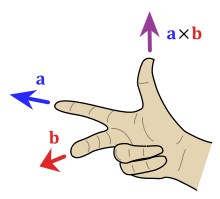
\includegraphics[height=4cm,width=1\textwidth,keepaspectratio]{resources/image9.png}
                \label{fig:resources/image9.png}
            \end{figure}
        \end{column}
    \end{columns}
\end{frame}

\begin{frame}[t]{Cross product}
    \framesubtitle{Video}
    \vspace{-0.6cm}
    \begin{figure}[H]
        \href{http://www.youtube.com/watch?v=h0NJK4mEIJU}{
            \centering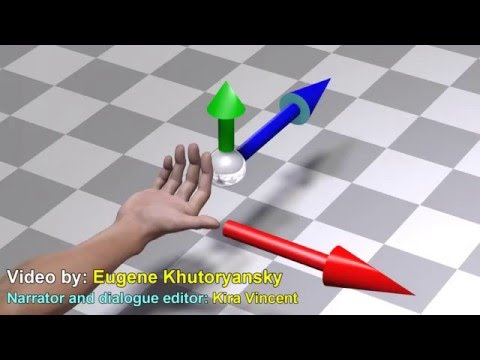
\includegraphics[height=6cm,width=1\textwidth,keepaspectratio]{resources/image8.jpg}}
        \label{fig:resources/image8.jpg}
    \end{figure}
\end{frame}

\begin{frame}[t]{Cross product: shoe polishing robot}
    \framesubtitle{Video}
    \vspace{-0.6cm}
    \begin{figure}[H]
        \href{https://docs.google.com/file/d/1VUmfmPc0qDTr51urLhXwV8uEXJ1DJfGC/preview}{
            \centering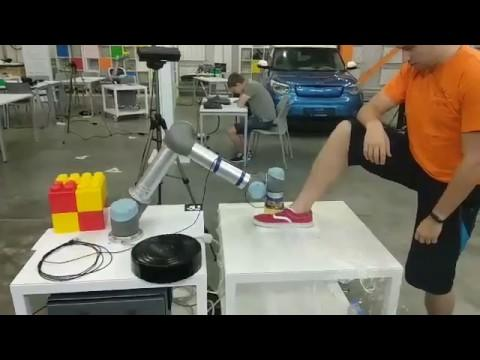
\includegraphics[height=6cm,width=1\textwidth,keepaspectratio]{resources/image12.jpg}}
        \label{fig:resources/image12.jpg}
    \end{figure}
\end{frame}

\begin{frame}[t]{How to calculate it?}
\framesubtitle{}
    \textbf{\LARGE Approaches for finding a full vector:}
    \begin{enumerate}
        \item Classical One
        \item Using skew-symmetric matrix
    \end{enumerate}
    \bigskip
    
    \textbf{\LARGE Approach for finding only magnitude:}
    \begin{enumerate}
        \item Geometrical representation
    \end{enumerate}
\end{frame}

\begin{frame}[t]{Classical One}
\framesubtitle{}
    \begin{align*}
        \vec{a} \times \vec{b} = \begin{vmatrix}
            \vec{i} & \vec{j} & \vec{k}\\ 
            a_{1} & a_{2} & a_{3}\\
            b_{1} & b_{2} & b_{3} 
       \end{vmatrix} = \vec{i}\begin{vmatrix} a_{2} & a_{3} \\ b_{2} & b_{3} \end{vmatrix} + 
       \vec{j}\begin{vmatrix} a_{1} & a_{3} \\ b_{1} & b_{3} \end{vmatrix} +
       \vec{k}\begin{vmatrix} a_{1} & a_{2} \\ b_{1} & b_{2} \end{vmatrix} \\
       \text{where, } \begin{vmatrix} a & b \\ c & d \end{vmatrix} = \det A = a \cdot d - b \cdot c
    \end{align*}
\end{frame}

\begin{frame}[t]{Using Skew-symmetric matrix}
\framesubtitle{}
    \vspace{-0.6cm}
    \begin{figure}[H]
        \centering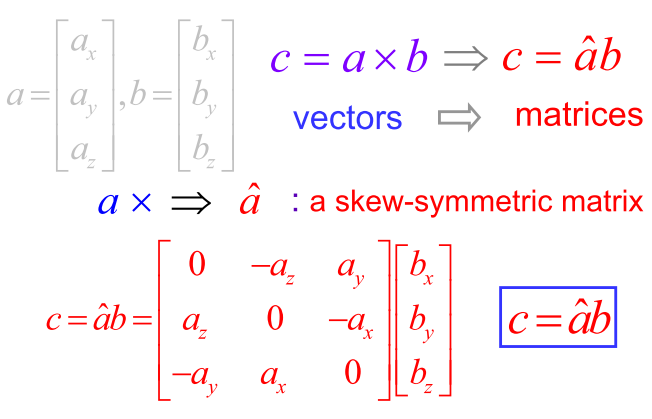
\includegraphics[height=6cm,width=1\textwidth,keepaspectratio]{resources/image13.png}
        \label{fig:resources/image13.png}
    \end{figure}
\end{frame}

\begin{frame}[t]{Geometrical representation}
\framesubtitle{}
\begin{columns}[T,onlytextwidth]
    \begin{column}{0.59\textwidth}
        $|\vec{a} \times \vec{b}| = |\vec{a}| |\vec{b}| \sin \alpha$ \\ 
        where $|\vec{a} \times \vec{b}|$ is an area of parallelogram \bigskip

        \textit{Tip:} The length or magnitude or norm of the vector a is denoted by $\|\vec{a}\|$ or, less commonly, $|\vec{a}|$, which is not to be confused with the absolute value (a scalar "norm"). \textit{In Russia, $|\vec{a}|$ is more popular}.
    \end{column}
    \begin{column}{0.39\textwidth}
        \begin{figure}[H]
            \centering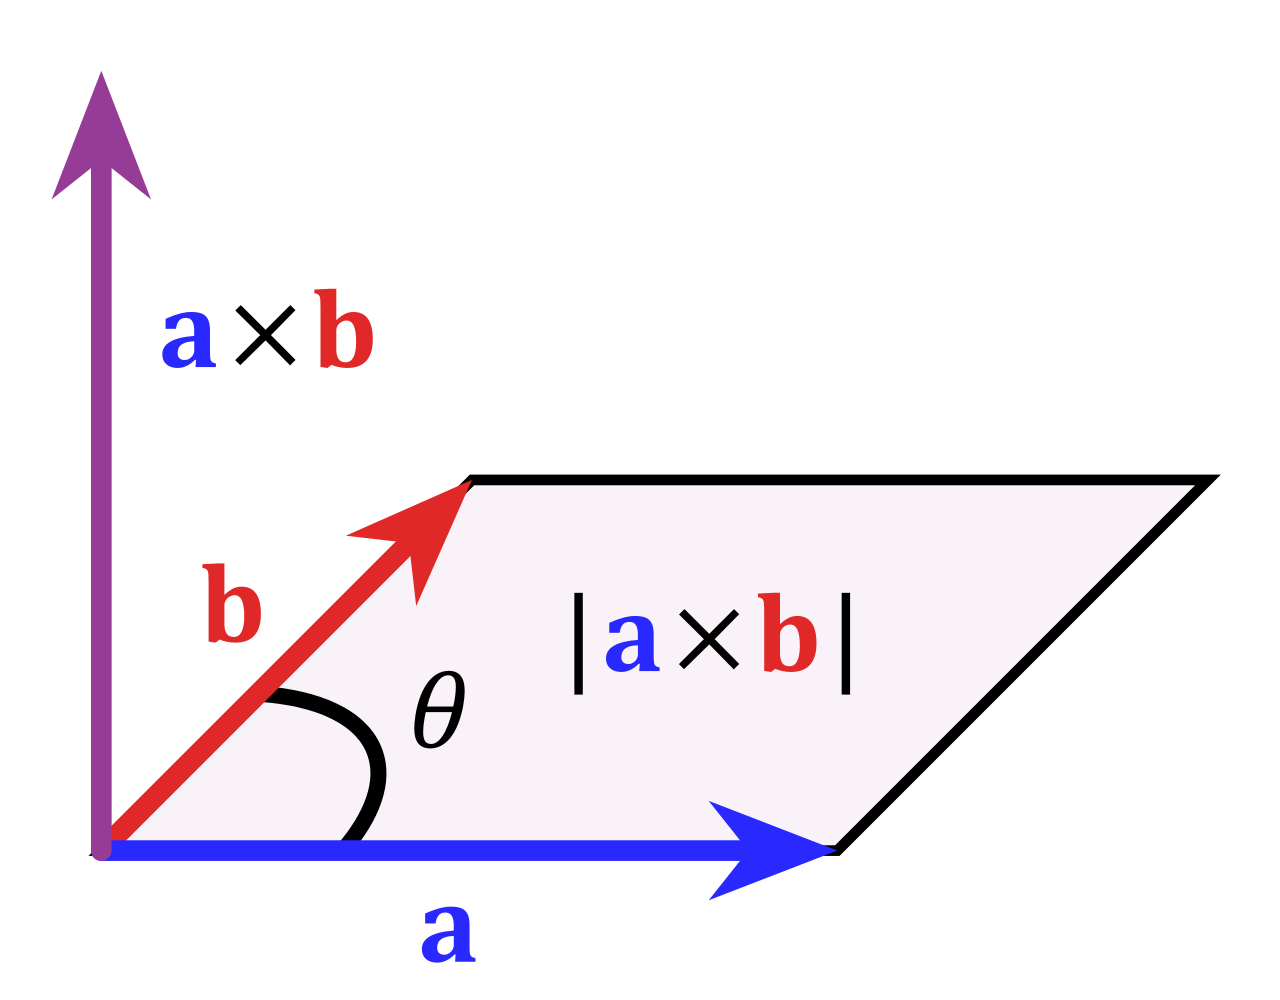
\includegraphics[height=5cm,width=1\textwidth,keepaspectratio]{resources/image15.png}
            % \caption{caption_name}
            \label{fig:resources/image15.png}
        \end{figure}
    \end{column}
\end{columns}
\end{frame}

\begin{frame}[t]{Cross product}
\framesubtitle{Case study}
    \textit{Task}: to find cross product between $\vec{a} = \begin{bmatrix}-2\\-2\\ 10\end{bmatrix}$ and $\vec{b}=\begin{bmatrix}-4\\1\\ 10\end{bmatrix}$

    \vspace*{0.2cm}
    \begin{columns}[T,onlytextwidth]
        \begin{column}{0.49\textwidth}
            \textbf{\LARGE Classical}
            \begin{multline*}
            \vec{a} \times \vec{b} = \begin{vmatrix}
                \vec{i} & \vec{j} & \vec{k}\\ 
                -2 & -2 & 10\\
                -4 & 1 & 10 
           \end{vmatrix} =\\ 
           = \vec{i}\begin{vmatrix} -2 & 10 \\ 1 & 10 \end{vmatrix} + 
           \vec{j}\begin{vmatrix} -2 & 10 \\ -4 & 10 \end{vmatrix} +
           \vec{k}\begin{vmatrix} -2 & -2 \\ -4 & 1 \end{vmatrix} = \begin{bmatrix}-30\\ -20\\ -10 \end{bmatrix}
           \end{multline*}
        \end{column}
        \begin{column}{0.49\textwidth}
            \textbf{\LARGE Skew-symmetric}
            \begin{align*}
                [\vec{a}\times]\vec{b}=\begin{bmatrix}
                    0 & -10 & -2 \\
                    10 & 0 & 2 \\ 
                    2 & -2  & 0 
                    \end{bmatrix}\begin{bmatrix}-4\\ 1\\ 10 \end{bmatrix}= \\ = \begin{bmatrix} -30\\-20\\ -10 \end{bmatrix}
            \end{align*}
        \end{column}
    \end{columns}
\end{frame}

\begin{frame}[t]{Cross product properties}
\framesubtitle{}
    \begin{enumerate}
        \item $\vec{a}\times\vec{b} = -(\vec{b}\times\vec{a})$
        \item $\vec{a}\times(\vec{b}+\vec{c})=\vec{a}\times\vec{b}+ \vec{a}\times\vec{c}$
        \item $(\vec{a}+\vec{b})\times\vec{c}=\vec{a}\times\vec{c}+ \vec{b}\times\vec{c}$
        \item $\lambda\vec{a}\times\vec{b}=\vec{a}\times\lambda\vec{b}=\lambda(\vec{a}\times\vec{b})$
        \item $\vec{a}\times\vec{a}=\vec{0}$
        \item $\vec{a}\times\vec{b}=\vec{0} \Leftrightarrow \vec{a}\parallel \vec{b}$
    \end{enumerate}
\end{frame}

\begin{frame}[t]{Task 1}
\framesubtitle{}
    Find cross product between $\vec{a}$ and $\vec{b}$, if:
    \begin{multicols}{2}
        \begin{enumerate}
            \item $\vec{a} = \begin{bmatrix}-1\\2\\1\end{bmatrix}$, $\vec{b}=\begin{bmatrix}7\\3\\5\end{bmatrix}$
            \item $\vec{a} = \begin{bmatrix}6\\9\\3\end{bmatrix}$, $\vec{b}=\begin{bmatrix}8\\8\\-5\end{bmatrix}$
            \item $\vec{a} = \begin{bmatrix}-9\\3\\-6\end{bmatrix}$, $\vec{b}=\begin{bmatrix}3\\5\\-8\end{bmatrix}$
            \item $\vec{a} = \begin{bmatrix}8\\3\\-9\end{bmatrix}$, $\vec{b}=\begin{bmatrix}7\\-1\\-6\end{bmatrix}$
        \end{enumerate}
    \end{multicols}
\end{frame}

\begin{frame}[t]{Task 2}
    \framesubtitle{}
    Simplify the expressions:
    \begin{enumerate}
        \item $(\vec{a}+\vec{b})\times(\vec{a}-\vec{b})$
        \item  $(3\vec{a} - \vec{b} - \frac{1}{3}\vec{c}) \times (2\vec{a} + \frac{3}{2}\vec{b} - 3\vec{c})$
    \end{enumerate}
    \uncover<2->{
        \alert{\Large Answer for <<1>>}
            \begin{figure}[H]
                \begin{subfigure}{0.65\textwidth}
                    \centering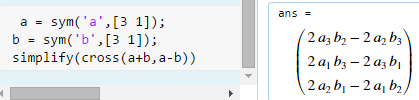
\includegraphics[height=3cm,width=1\textwidth,keepaspectratio]{resources/image26.png}
                    % \caption{capture1}
                    \label{fig:resources/image26.png}
                \end{subfigure}
                \begin{subfigure}{0.33\textwidth}
                    \centering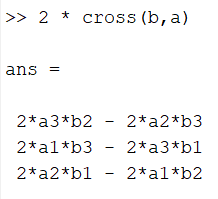
\includegraphics[height=3cm,width=1\textwidth,keepaspectratio]{resources/image21.png}
                    \label{fig:resources/image21.png}
                \end{subfigure}
            \end{figure}
    }
\end{frame}

\begin{frame}[t]{Task 3}
\framesubtitle{}
A triangle is constructed on vectors $\vec{a} = \begin{bmatrix}2\\4\\-1\end{bmatrix},\ \vec{b} = \begin{bmatrix}-2\\1\\1\end{bmatrix}$.

It is needed to
\begin{enumerate}
    \item Find the area of the triangle.
    \item Find the altitudes of this triangle.
\end{enumerate}
\end{frame}

\begin{frame}[t]{Lab objectives, 2nd part}
\framesubtitle{}
    \begin{enumerate}
        \item What does dot product mean?
        \item How to calculate it?
        \item How to use it?
    \end{enumerate}
\end{frame}

\begin{frame}[t]{Dot product}
\framesubtitle{Definition}
The result of \textbf{dot product / inner product} $\vec{a} \cdot \vec{b}= (\vec{a},\vec{b}) = \vec{a}^T\vec{b} = \sum a_i b_i = a_1 b_1 + a_2 b_2 + a_3 b_3 $  between $\vec{a}$ and $\vec{b}$ is a \textbf{scalar}. 
\medskip

Geometrically --- $\vec{a} \cdot \vec{b} = |\vec{a}| |\vec{b}| \cos \beta$ --- measure of how similar two vectors are.
\end{frame}

\begin{frame}[t]{Dot product}
    \framesubtitle{Video}
    \vspace{-0.6cm}
    \begin{figure}[H]
        \href{http://www.youtube.com/watch?v=TBpDMLCC2uY&t=65}{
            \centering
\includegraphics[height=6cm,width=1\textwidth,keepaspectratio]{resources/image24.jpg}}
        \label{fig:resources/image24.jpg}
    \end{figure}
\end{frame}

\begin{frame}[t]{Tasks 4 and 5}
\framesubtitle{}
\begin{enumerate}
    \item Solve $|\vec{a}|^2 - 2\sqrt{3}\vec{a} \cdot \vec{b} - 7 |\vec{b}|^2$, where $ |\vec{a}| = 4,\ |\vec{b}| = 1,\ \angle(\vec{a},\vec{b}) = 150^\circ$
    \item Find the angle between $\vec{a}=\begin{bmatrix} 1\\ -1\\ 1 \end{bmatrix},\ \vec{b}=\begin{bmatrix} -5\\ -1\\ -1 \end{bmatrix}$
\end{enumerate}
\end{frame}

\begin{frame}[t]{Task 6}
    \framesubtitle{}
    \only<1>{
        All three vectors $\vec{a},\ \vec{b},\ \vec{c}$ have length of $3$ and $\vec{a}+\vec{b}+\vec{c} = \vec{0}$. \medskip

        Find $\vec{a} \cdot \vec{b} + \vec{b} \cdot \vec{c} + \vec{c} \cdot \vec{a} $
    }
    \only<2>{
        \alert{\Large Answer: $-\dfrac{27}{2}$}
        \begin{figure}[H]
            \centering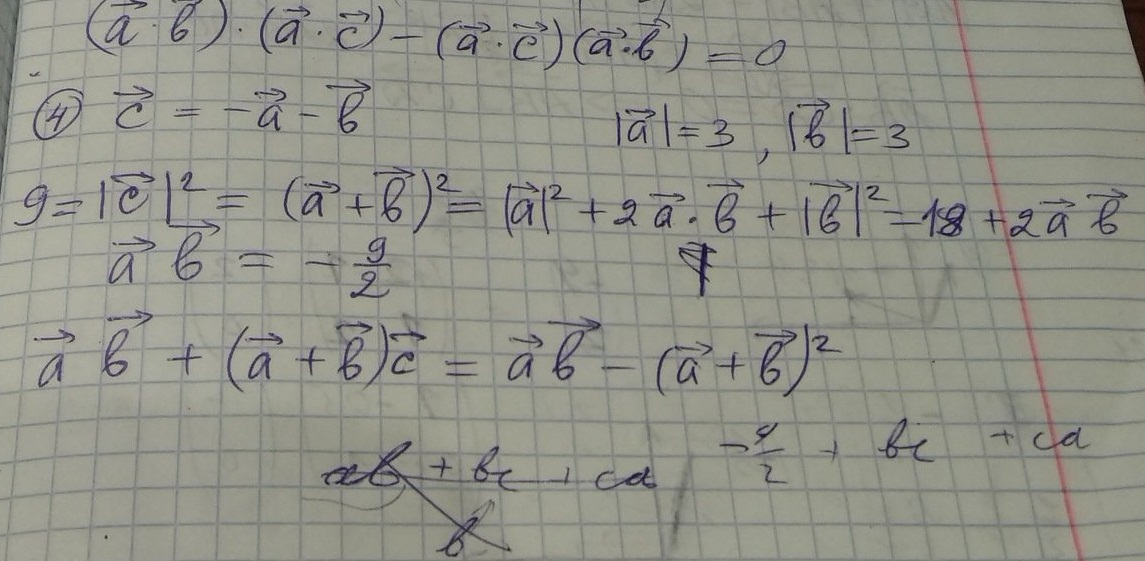
\includegraphics[height=4cm,width=1\textwidth,keepaspectratio]{resources/image25.jpg}
            \caption*{Pure math solution}
            \label{fig:6ans.png}
        \end{figure}
    }
\end{frame}

\begin{frame}[t]{Dot and cross product possible application}
    \framesubtitle{Video}
    \vspace{-0.6cm}
    \begin{figure}[H]
        \href{http://www.youtube.com/watch?v=_PZ8V1ZDAc8}{
            \centering
\includegraphics[height=6cm,width=1\textwidth,keepaspectratio]{resources/image31.jpg}}
        \label{fig:resources/image31.jpg}
    \end{figure}
\end{frame}

\begin{frame}[t]{Task 7}
    \framesubtitle{}
    \only<1>{
        There are two vectors on some basis $\vec{a}=\begin{bmatrix} x\\ 1-x \end{bmatrix},\ \vec{b}=\begin{bmatrix} x^2-2x\\ x^2-2x+1 \end{bmatrix}$.

        It is needed to find $x$, when:
        \begin{enumerate}
            \item Vectors are collinear
            \item They have the same direction
        \end{enumerate}
     }
    \only<2>{
        \begin{figure}[H]
            \centering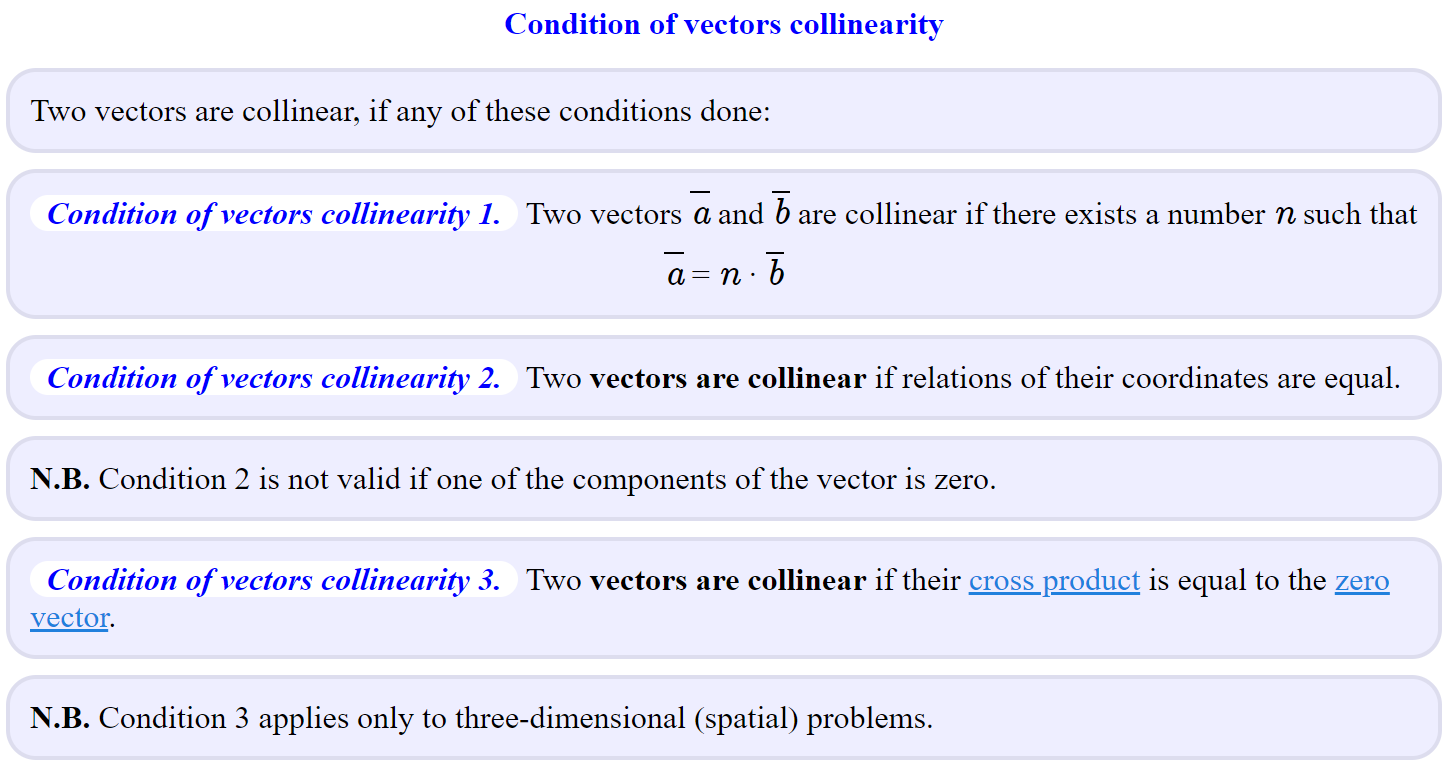
\includegraphics[height=5.5cm,width=1\textwidth,keepaspectratio]{resources/image37.png}
            % \caption{caption_name}
            \label{fig:resources/image37.png}
        \end{figure}
    }
\end{frame}

\begin{frame}[t]{Task 8}
    \framesubtitle{At home}
    \only<1>{
        The edges of cube $ABCDA_1B_1C_1D_1$ have length of $1$. $P$ is a midpoint of $CC_1$ and $Q$ is a center of face $AA_1B_1B$. Points $M$ and $N$ belong to lines $AD$ and $A_1B_1$ respectively, and at that $MN$ intersects with $PQ$ and is perpendicular to it. Find $MN$.
     }
    \only<2>{
        \framesubtitle{Geogebra with link}
        \vspace{-0.4cm}
        \begin{figure}[H]
            \href{https://www.geogebra.org/classic/cmutqjtn}{
                \centering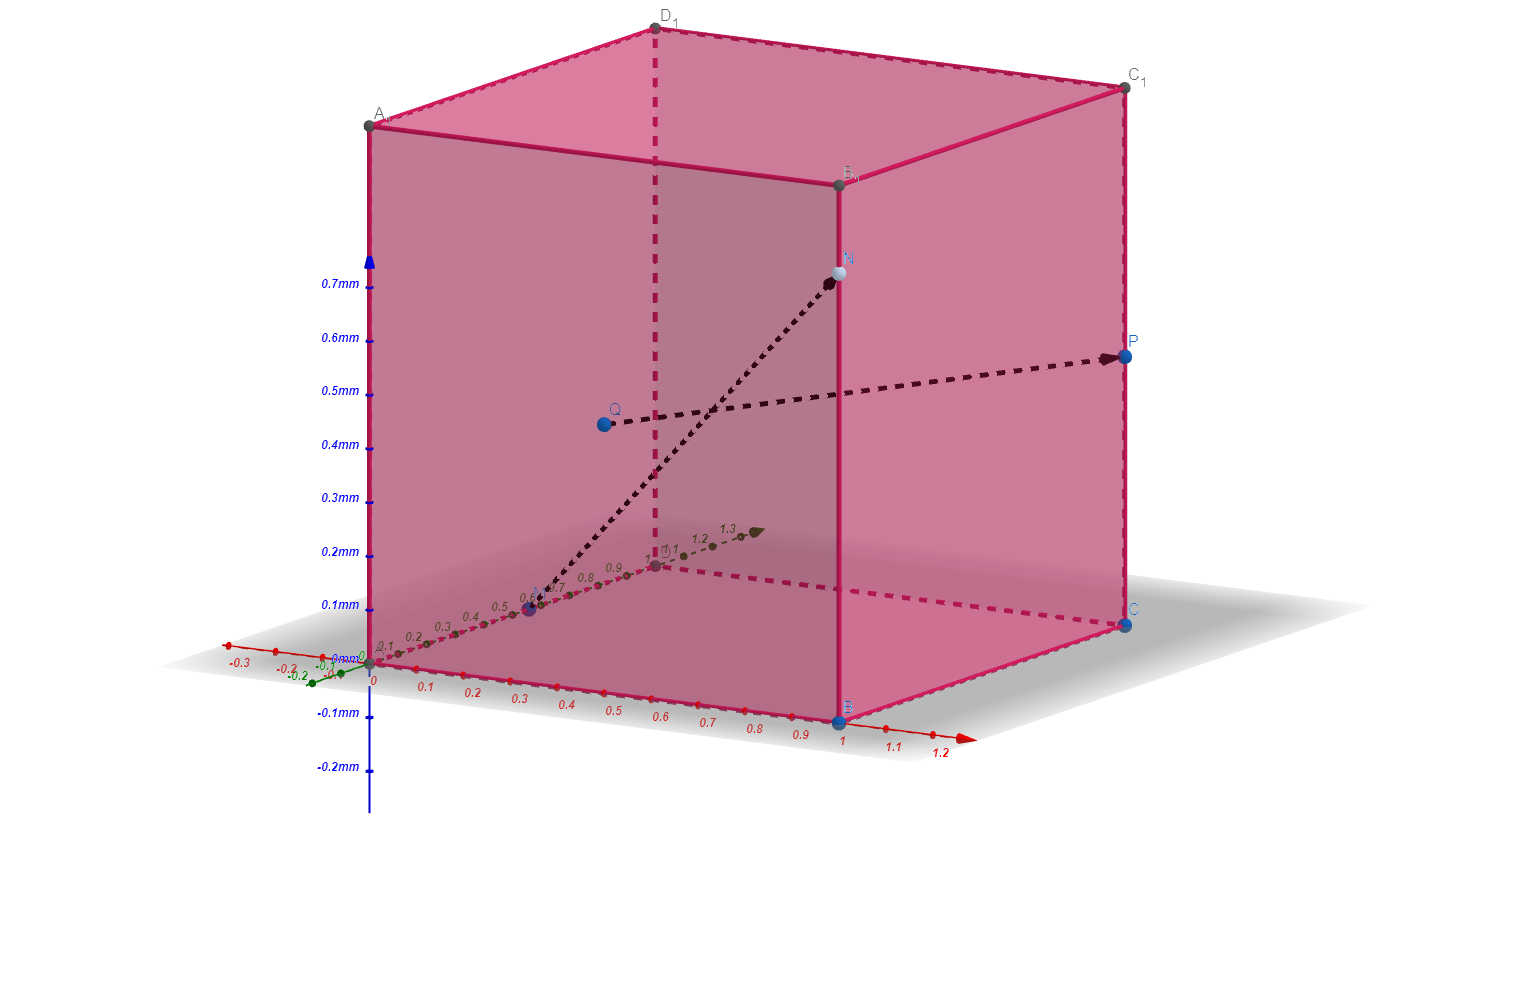
\includegraphics[height=6cm,width=1\textwidth,keepaspectratio]{resources/image33.png}}
            \label{fig:resources/image33.png}
        \end{figure}
    }
    \only<3>{
        \framesubtitle{A hint}
        It is needed to make 2 equations: 1 for perpendicularity, 2nd --- intersection. Think about amount of unknowns and possible equations.
        \begin{figure}[H]
            \centering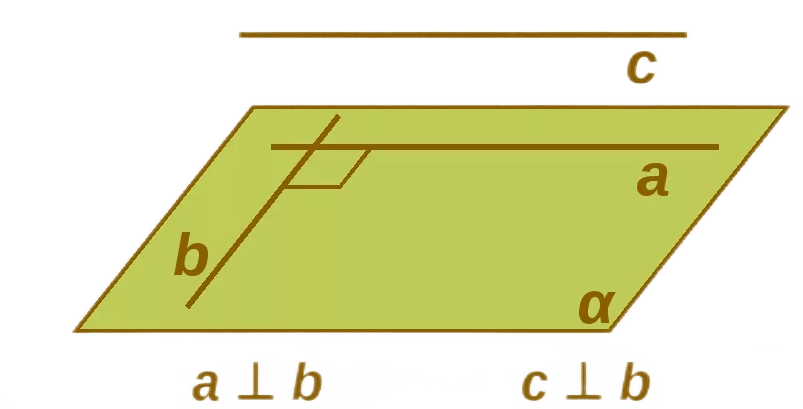
\includegraphics[height=4cm,width=1\textwidth,keepaspectratio]{resources/image35-transformed.png}
            % \caption{caption_name}
            \label{fig:resources/image35-transformed.png}
        \end{figure}
    }
\end{frame}

\begin{frame}[t]{Reference material}
    \framesubtitle{}
    \begin{itemize}
        \item \href{https://youtu.be/eu6i7WJeinw?si=f1X1RMej4nH6WEup}{Cross products | Chapter 10, Essence of linear algebra - YouTube}
        \item \href{https://youtu.be/LyGKycYT2v0?si=AAUk7OolGJPaQT3S}{Dot product | Chapter 9, Essence of linear algebra - YouTube}
        \item \href{https://onlinemschool.com/math/library/vector/multiply1/}{Cross product of two vectors - OnlineMSchool}
        \item \href{http://www.mathprofi.ru/vektornoe_proizvedenie_vektorov_smeshannoe_proizvedenie.html}{Векторное произведение векторов - Матпрофи}
    \end{itemize}
\end{frame}

\fbckg{fibeamer/figs/last_page.png}
\frame[plain]{}

\end{document}